\documentclass{article}
\usepackage[utf8]{inputenc}

\usepackage{graphicx} %package to manage images
\graphicspath{ {./Bilder/} }

\usepackage[rightcaption]{sidecap}

\usepackage{wrapfig}

\title{Service Vehicles Network}
\author{Lukas.Ostrzinski }
\date{June 2020}

\begin{document}

\maketitle

\section{Introduction}

\subsection{Motivation}
Smart Cities is an futuristic concept which has become more and more relevant recently. Because of this, infrastructure like transportation or emergency systems will become more automatic and controlled over an whole server system. 
\newline
Barcelona has always been included in the top 10 rankings when it comes to Smart cities. It has a well-documented history in this area and today integrates intelligent sensors and big data analyzed in a wide variety of areas, from parking lot management and traffic management to garbage disposal, management of air quality and irrigation of green areas. [1]

\subsection{Emergency Services in Smart Cities}
If police, firefighters and ambulances could use this technology, it would be a lot easier for them to react to an emergency like an car crash or other kinds of emergency situations. Automation could make the process of calling an ambulance more efficient and faster. For example, a car which was involved in an car crash could call the ambulance automatically. This would be especially helpful when the driver cannot call the ambulance because he is unconscious or unable to access his phone.




\section{Concept}
The aim of the project is to implement an program which queries the position of an emergency and the type of emergency. Depending on the type of the emergency, the program sends the right vehicle to the position. 
There are 3 kinds of vehicles: ambulances, firetrucks and police cars.
\newline
The program gets the information about the position and the type of the emergency from a server. The program tells the server when it sends the requested vehicle to the location of the emergency and again when the vehicles arrive and leave this location. 

\clearpage
My idea to implement my part of the system was to write 3 programs in which each of them take cares of one of the emergency response vehicles: police cars, firetrucks and ambulances. The structure of each one will be only minimally different. First, I will describe the functional requirements.
\newline
Firstly, the program needs to get the information about the coordinates from the place of operation and determine which of these vehicles needs to be sent to this place. When the program gets this information, it will send an conformation back to the server and say that the vehicle will drive to the place operation. 
\newline

\begin{figure}[htp]
    \centering
\includegraphics[width=12cm, height=6cm]{images/Ostrzinski/com2}
    \caption{Conformation vehicle to server}
    \label{fig:GALAXY}
\end{figure}

When the vehicle arrives at the place of operation, the program sends an another message to the server indicating that the vehicles have arrived. When the Vehicles leave the location, the server will get another message from the program. After that, when the vehicles returned to their base, the program gives a last message to the server that these vehicles are available and can be used again.
\newline
\newline
Now the nonfunctional requirements: Every vehicle has a specific number of people it can carry. The police cars can carry 2 people, 1 driver/officer and 1 normal officer. The firetrucks can carry 9 people, with 1 driver/firefighter, 1 head of operations and 7 normal firefighters. The ambulances can carry 2 people, 1 driver and 1 specialist/doctor. 
\newline
The conformation for the information and departure of the vehicles is not allowed to be longer than 1 minute. The time until the ambulance arrives at the place of operation needs to be under 8 minutes. The firetruck needs to arrive in under 20 minutes at the place of operation. And the police cars need to arrive there in under 15 minutes. 
\newline
The conformation of the arrival needs to be sent within 2 minutes of the vehicles' arrival, and the confirmation of the departure also needs to be sent within 2 minutes of the vehicles' departure from the place of operation.

\clearpage
As a better overview, here is a list of all the requirements.
\newline
\newline
\begin{figure}[htp]
    \centering
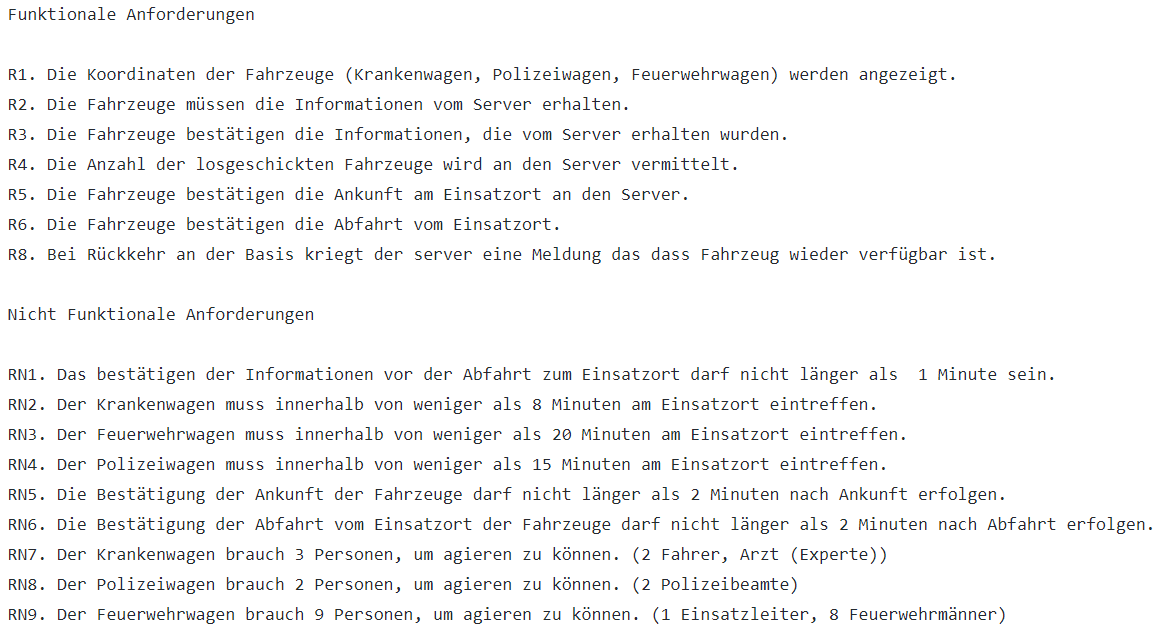
\includegraphics[width=14cm, height=8cm]{images/Ostrzinski/RL}
    \caption{Requirements list}
    \label{fig:GALAXY}
\end{figure}
\clearpage

And here is an better visualization with the Use-Case diagram.
\newline
\newline
\begin{figure}[htp]
    \centering
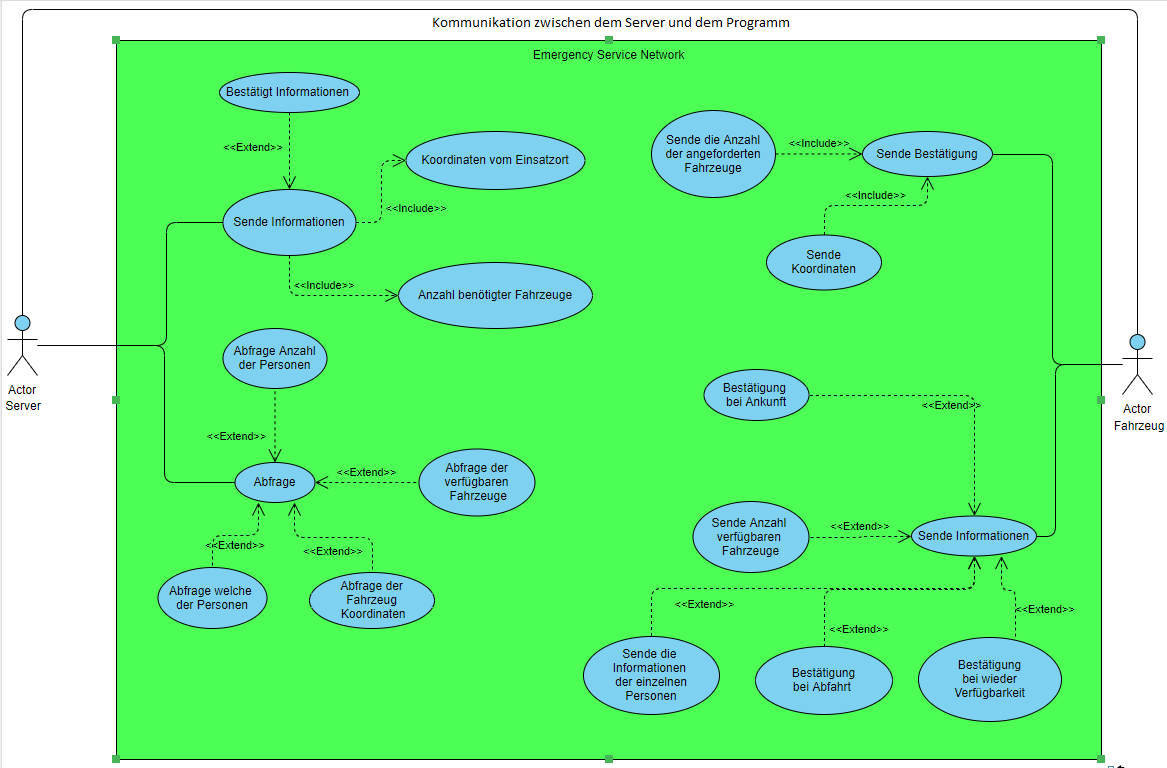
\includegraphics[width=16cm, height=10cm]{images/Ostrzinski/UCD}
   \caption{Use-Case Diagram}
    \label{fig:GALAXY}
\end{figure}
\newline
\newline
This Use-Case diagram is divided into two parts, the server part and the vehicle part.
\newline
The server part shows what kind of questions it can ask the program and also which kinds of information it can give the program. These are the coordinates for the place of operation, which vehicles need to be sent and how many vehicles need to be sent.
\newline
The program/vehicle part shows the confirmations which the program gives to the server in specific situations. 
\newline
The program also sends information to the server like the when a vehicle arrives at the place of operation, when the vehicle leaves this place again and when the vehicle is back at its base and available to be sent out again.
\clearpage

\section{Implementation}


The implementation is written in Python. As already mentioned, each type of vehicle has its own program, so one for the police cars, one for the firetrucks and one for the ambulances. 
\newline
In order to leave some time between the messages and actions, there is a file for each vehicle which generates random times for how long the vehicle needs to arrive at the place of operation and leave it again, and this file is called "waiter."

\subsection{Main Program}
To let the program work, we need to start the main program and waiter first before the server starts. When this happens, the server get first a message about how many vehicles are available. Now the server can type in its information which includes the name of the person who needs help, which vehicles need to be sent and the case.
 Requirement R1, R2, suffused.
\begin{figure}[htp]
    \centering
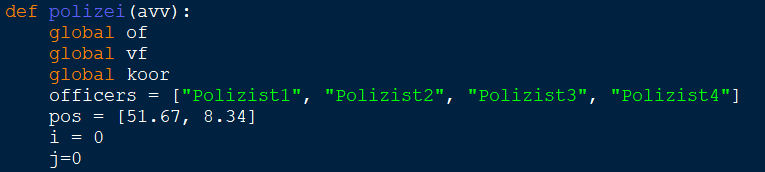
\includegraphics[width=12cm, height=4cm]{images/Ostrzinski/I1}
   \caption{Method polizei 1-4}
    \label{fig:GALAXY}
\end{figure}
\newline
\newline
This method is used to create police cars, with the maximum amount of vehicles based on a variable called "avv" and the number of names listed, in this case, officers. The method can create two cars because "avv" is currently 2 and officers have only 4 names listed, since each car needs two names to be created.
\newline
The variable "of" is a list in which the names, the ID and the coordinates of all the cars are saved.
The variable "vf" stores the number of vehicles which are available.
In the last variable "koor" are the randomly generated coordinates from the vehicles saved as well as the new coordinates when the vehicle changes position.
\newline
The "global" before each of these variables makes it possible to also save the variables outside of the method. Requirement RN7, RN8, RN9 suffused.

\clearpage
\begin{figure}[htp]
    \centering
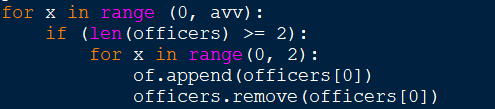
\includegraphics[width=10cm, height=2cm]{images/Ostrzinski/I2}
   \caption{Method polizei 2-4}
    \label{fig:GALAXY}
\end{figure}
\newline
\newline
The first "for loop" is used to run the code a given number of times based on "avv". 
The "if" check ifs there are names left.
\newline
The second "for loop" runs the code twice. Inside the loop, the first name on the officer list is added to "of," and then this name gets removed from the officer list. 
\newline
\newline
\begin{figure}[htp]
    \centering
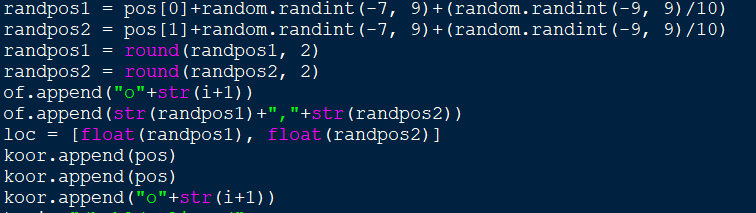
\includegraphics[width=12cm, height=4cm]{images/Ostrzinski/I3}
   \caption{Method polizei 3-4}
    \label{fig:GALAXY}
\end{figure}
\newline
\newline
In this part of the of the method, randomly generated coordinates get assigned to the vehicles.
After that, an ID is assigned to the vehicles. The IDs for police cars always start with "o,"  firetrucks start with "s" and ambulances start with "k."

\clearpage
\begin{figure}[htp]
    \centering
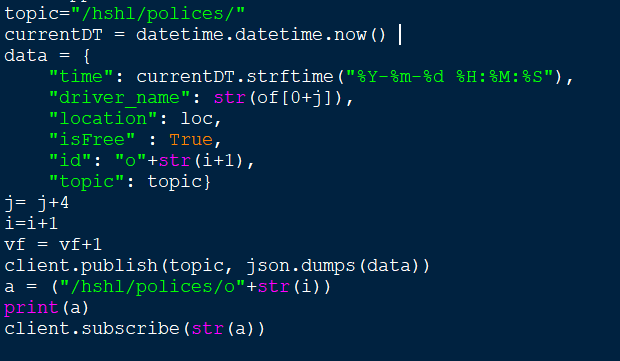
\includegraphics[width=12cm, height=6cm]{images/Ostrzinski/I4}
   \caption{Method polizei 4-4}
    \label{fig:GALAXY}
\end{figure}
\newline
\newline
This part of the method saves the topic "/hshl/polices/" and the current time and date.
Then the generated vehicle is saved as a Json data and is sent to the given topic.
Now the program subscribes to the vehicle ID. 

\begin{figure}[htp]
    \centering
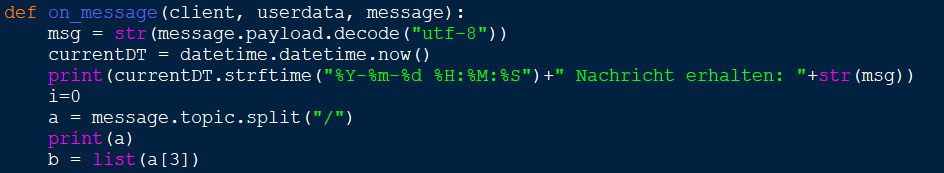
\includegraphics[width=14cm, height=4cm]{images/Ostrzinski/I5}
   \caption{Method on\_message 1-2}
    \label{fig:GALAXY}
\end{figure}
\newline
\newline
The program waits for a message and then calls this method "on\_message".
\newline
After it gets a message, the method converts this message into a string and displays it along with the topic. 

\clearpage
\begin{figure}[htp]
    \centering
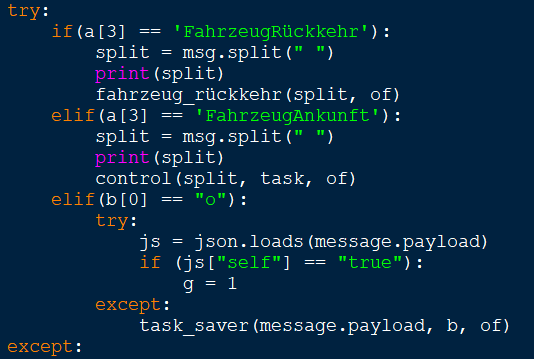
\includegraphics[width=8cm, height=4cm]{images/Ostrzinski/I6}
   \caption{Method on\_message 2-2}
    \label{fig:GALAXY}
\end{figure}
\newline
\newline
In this part of the method, "on\_message" decides which method should be called upon based on the topic of the message.
\newline
\begin{figure}[htp]
    \centering
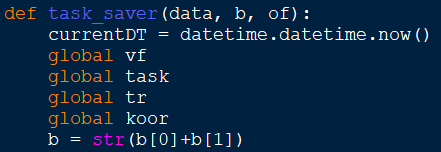
\includegraphics[width=8cm, height=2cm]{images/Ostrzinski/I7}
   \caption{Method task\_saver 1-2}
    \label{fig:GALAXY}
\end{figure}
\newline
\newline
The method "task\_saver" checks if a vehicle is available or has already been sent to the place of operation.
\newline
The variable "task" is the list of the information from the server like coordinates, the names of the people who need help and the case from this person (e.g. heart attack, open wounds).
\newline
The variable "tr" makes sure the method runs in the right order.
In the variable "b," the ID is saved.

\begin{figure}[htp]
    \centering
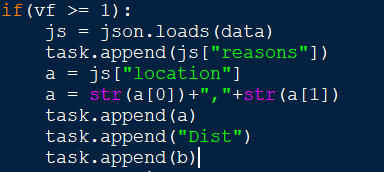
\includegraphics[width=9cm, height=3cm]{images/Ostrzinski/I8}
   \caption{Method task\_saver 2-2}
    \label{fig:GALAXY}
\end{figure}
\newline
This part of the method "task\_saver" is only executed when at least one vehicle "vf" is available and when the vehicle is not in use yet.
\newline
If that is not the case, this method will say "Vehicle not available."
\newline

\begin{figure}[htp]
    \centering
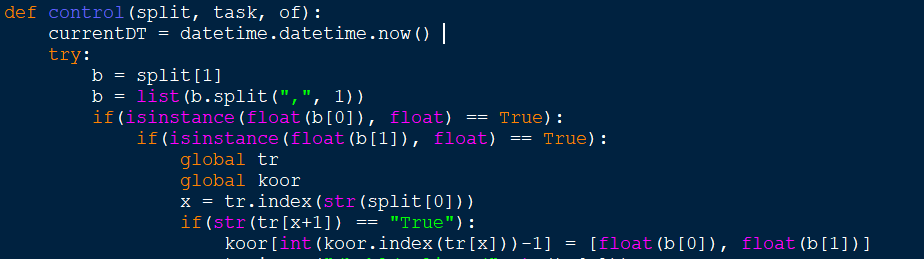
\includegraphics[width=12cm, height=4cm]{images/Ostrzinski/I9}
   \caption{Method control}
    \label{fig:GALAXY}
\end{figure}
\newline
\newline
The method "control" says that the vehicle now arrives at the place of operation and give this information to the server together with the current coordinates. It also checks if the received information is correct. Requirement R5 suffused.


\begin{figure}[htp]
    \centering
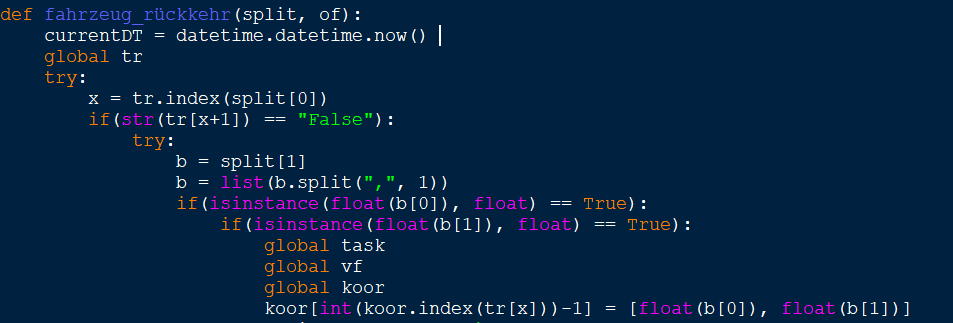
\includegraphics[width=12cm, height=4cm]{images/Ostrzinski/I10}
   \caption{Method fahrzeug\_rückkehr}
    \label{fig:GALAXY}
\end{figure}

The method "fahrzeug\_rückkehr" gets a message that the vehicle has returned from the operation and makes the vehicle available again for the next case.  Requirement R8 suffused.

\subsection{Waiter}
The waiter communicates with main program and generates a random number from 5 to 10. The waiter gets a message (vehicle sent) from the main program and waits then 5 to 10 seconds depending on which number gets generated and gives the message back to the main program (vehicle arrived). Then it again generates a number from 5 to 10, waiting again depending on this  randomly generated number and again sends a message to the main program (vehicle returned).  Requirement RN2, RN3, RN4  suffused.

\section{Conclusion}
For this project, I implemented 3 main files, 1 for the police, 1 for the ambulance and 1 for the firefighter, and each of them act independently.
\newline
Each these also have their own file for waiting times in between the "waiter."  The only difference between them is the number of people which they have included. 
\newline
In the end, not every requirement was achievable since I was not alone, and the server was implemented by another person; that is why these conformation requirements specifically are not all included in this program.
Additionally, this would restrict the performance too much, so we decided not to write these functions into the main program. That means the requirements R3, R4, R5, R6, RN1, RN5 and RN6 are not included in the implementation and suffused.
\newline
For the future, it would be good to communicate more with the other people who were included in the project. First I had a lot of these conformation in the implementation, and then when I asked about these things, I found out that the others did not put them in their programs. This is why I needed to change the implementation a lot in between. This became better in the end, but it would had be a lot better from the beginning.

\begin{thebibliography}{9}
\bibitem{}
Urban Hub - People Shaping Cities. 
\textit{The \LaTeX\ Companion}. 
Smart City 3.0 – Fragen Sie Barcelona nach der nächsten Generation von Smart City.



\end{thebibliography}
\end{document}
